% Comentarios para Plos {{{
% The manuscript LaTeX source should be contained within a single file (do not use \input, \externaldocument, or similar commands).
%
% -- FIGURES AND TABLES
%
% Please include tables/figure captions directly after the paragraph where they are first cited in the text.
%
% DO NOT INCLUDE GRAPHICS IN YOUR MANUSCRIPT
% - Figures should be uploaded separately from your manuscript file. 
% - Figures generated using LaTeX should be extracted and removed from the PDF before submission. 
% - Figures containing multiple panels/subfigures must be combined into one image file before submission.
% For figure citations, please use "Fig" instead of "Figure".
% See http://journals.plos.org/plosone/s/figures for PLOS figure guidelines.
%
% Tables should be cell-based and may not contain:
% - spacing/line breaks within cells to alter layout or alignment
% - do not nest tabular environments (no tabular environments within tabular environments)
% - no graphics or colored text (cell background color/shading OK)
% See http://journals.plos.org/plosone/s/tables for table guidelines.
%
% For tables that exceed the width of the text column, use the adjustwidth environment as illustrated in the example table in text below.
%
% % % % % % % % % % % % % % % % % % % % % % % %
%
% -- EQUATIONS, MATH SYMBOLS, SUBSCRIPTS, AND SUPERSCRIPTS
%
% IMPORTANT
% Below are a few tips to help format your equations and other special characters according to our specifications. For more tips to help reduce the possibility of formatting errors during conversion, please see our LaTeX guidelines at http://journals.plos.org/plosone/s/latex
%
% When adding superscript or subscripts outside of brackets/braces, please group using {}.  For example, change "[U(D,E,\gamma)]^2" to "{[U(D,E,\gamma)]}^2". 
%
% Do not use \cal for caligraphic font.  Instead, use \mathcal{}
% }}}

\documentclass[10pt,letterpaper]{article} % {{{
\usepackage[top=0.85in,left=2.75in,footskip=0.75in]{geometry}

\usepackage{amsmath,amssymb}
\usepackage{changepage}
\usepackage[utf8x]{inputenc}
% \usepackage{textcomp,marvosym}
\usepackage{cite}
% Use nameref to cite supporting information files (see Supporting Information section for more info)
\usepackage{nameref,hyperref}
\usepackage[right]{lineno}

% ligatures disabled
\usepackage{microtype}
\DisableLigatures[f]{encoding = *, family = * }

\newcommand{\eref}[1]{Eq.~(\ref{#1})}
\newcommand{\Eref}[1]{Eq.~(\ref{#1})}
\newcommand{\fref}[1]{Fig.~\ref{#1}}
\newcommand{\Fref}[1]{Fig.~\ref{#1}}
% color can be used to apply background shading to table cells only
\usepackage[table]{xcolor}
\usepackage{array}
\usepackage{caption}
\usepackage{multirow}
\usepackage{booktabs}
\usepackage{graphicx}
\usepackage{pbox}
\usepackage{makecell}
\usepackage{boldline,multirow}

\usepackage{soul}

\usepackage{pdfpages}
\usepackage{tcolorbox}
\usepackage{colortbl}

\usepackage{booktabs}

\usepackage[draft,inline,nomargin]{fixme} \fxsetup{theme=color}
\FXRegisterAuthor{jm}{jmm}{\color{purple}Josue}
\FXRegisterAuthor{nr}{nrr}{\color{brown}{NR}}
\FXRegisterAuthor{cp}{acp}{\color{blue}CP}
\FXRegisterAuthor{cg}{cgg}{\color{red}CG}

\definecolor{C1-EN}{RGB}{0,132,170}
\definecolor{C1-FR}{RGB}{255,117,0}
\definecolor{C1-GE}{RGB}{134,0,179}
\definecolor{C1-IT}{RGB}{49,129,6}
\definecolor{C1-SP}{RGB}{162,0,0}

\newcolumntype{+}{!{\vrule width 2pt}}

% create \thickcline for thick horizontal lines of variable length
\newlength\savedwidth
\newcommand\thickcline[1]{%
	\noalign{\global\savedwidth\arrayrulewidth\global\arrayrulewidth 2pt}%
	\cline{#1}%
	\noalign{\vskip\arrayrulewidth}%
	\noalign{\global\arrayrulewidth\savedwidth}%
}

% \thickhline command for thick horizontal lines that span the table
\newcommand\thickhline{\noalign{\global\savedwidth\arrayrulewidth\global\arrayrulewidth 2pt}%
	\hline
	\noalign{\global\arrayrulewidth\savedwidth}}


% Remove comment for double spacing
%\usepackage{setspace} 
%\doublespacing

% Text layout
\raggedright
\setlength{\parindent}{0.5cm}
\textwidth 5.25in 
\textheight 8.75in

% Bold the 'Figure #' in the caption and separate it from the title/caption with a period
% Captions will be left justified
\usepackage[aboveskip=1pt,labelfont=bf,labelsep=period,justification=raggedright,singlelinecheck=off]{caption}
\renewcommand{\figurename}{Fig}

% Use the PLoS provided BiBTeX style
\bibliographystyle{plos2015}

% Remove brackets from numbering in List of References
\makeatletter
\renewcommand{\@biblabel}[1]{\quad#1.}
\makeatother



% Header and Footer with logo
\usepackage{lastpage,fancyhdr,graphicx}
\usepackage{epstopdf}
%\pagestyle{myheadings}
\pagestyle{fancy}
\fancyhf{}
%\setlength{\headheight}{27.023pt}
%\lhead{\includegraphics[width=2.0in]{PLOS-submission.eps}}
\rfoot{\thepage/\pageref{LastPage}}
\renewcommand{\headrulewidth}{0pt}
\renewcommand{\footrule}{\hrule height 2pt \vspace{2mm}}
\fancyheadoffset[L]{2.25in}
\fancyfootoffset[L]{2.25in}
\lfoot{\today}

%% Include all macros below

\newcommand{\lorem}{{\bf LOREM}}
\newcommand{\ipsum}{{\bf IPSUM}}

%\FXRegisterAuthor{cg}{cgg}{\color{red}CG}

%% END MACROS SECTION

% }}}
\begin{document}
% Autores, titulo y otros {{{
\vspace*{0.2in}

% Title must be 250 characters or less.
\begin{flushleft}
{\Large
\textbf\newline{Statistical analysis of word flow among five Indo-European languages} % Please use "sentence case" for title and headings (capitalize only the first word in a title (or heading), the first word in a subtitle (or subheading), and any proper nouns).
}
\newline
Josué Ely Molina  \ddag\textsuperscript{1,2}, %\textsuperscript{1,2\Yinyang},
Jorge Flores      \dag \textsuperscript{2}, %\textcurrency},
Carlos Gershenson \textsuperscript{3,4,5},
% Sergio Sanchez    \textsuperscript{6},\\
Carlos Pineda     \ddag\textsuperscript{2,*}    % \textsuperscript{2\Yinyang},
% 


\bigskip
\newcommand{\unam}{Universidad Nacional Aut\'{o}noma de M\'{e}xico, Mexico City, 01000, Mexico}
\textbf{1} Facultad de Ciencias, \unam \\
\textbf{2} Instituto de F\'{\i}sica, \unam \\
\textbf{3} Instituto de Investigaciones en Matem\'{a}ticas Aplicadas y Sistemas, \unam \\
\textbf{4} Centro de Ciencias de la Complejidad, \unam \\
\textbf{5} Santa Fe Institute. 1399 Hyde Park Rd., Santa Fe, NM 87501, USA\\
% \textbf{6} 
% Maestr\'{\i}a en Ciencias de la Complejidad, 
% Universidad Aut\'{o}noma de la Ciudad de M\'{e}xico,
% Mexico City, Mexico
% \\
\bigskip
\ddag These authors contributed equally to this work.
\dag Deceased \\
* carlospgmat03@gmail.com
\end{flushleft}
% }}}
\section*{Abstract} % {{{
% Please keep the abstract below 300 words

A recent increase in computational processing, has allowed the possibility to perform different linguistic studies with large datasets. Here we use the Google Books Ngram dataset to analyze word flow among English, French, German, Italian, and Spanish. We study what we define as ``migrant words'', a type of loanwords that do not change their spelling. We quantify migrant words from one language to another for different decades, and notice that most migrant words can be aggregated in semantic fields and associated to historic events. We also study some properties of accumulated migrant words and their rank dynamics. We propose a measure of \emph{use} of migrant words that could be used as a proxy of cultural influence. Our methodology is not exempt of caveats, but our results are encouraging to promote further studies in this direction.

%A recent increase in data availability has allowed the possibility to perform different linguistic studies with bi. Here we use the Google Books Ngram dataset to analyze word flow among English, French, German, Italian, and Spanish. We study what we define as ``migrant words'', a type of loanwords that do not change their spelling. We quantify migrant words from one language to another for different decades, and notice that most migrant words can be aggregated in semantic fields and associated to historic events. We also study some properties of accumulated migrant words and their rank dynamics. We propose a measure of \emph{use} of migrant words that could be used as a proxy of cultural influence. Our methodology is not exempt of caveats, but our results are encouraging to promote further studies in this direction.


% }}}
% \linenumbers
% Use "Eq" instead of "Equation" for equation citations.
% For figure citations, please use "Fig" instead of "Figure".
\section*{Introduction} % {{{

% {\color{C1-EN} {C1-EN}}
% {\color{C1-FR} {C1-FR}}
% {\color{C1-GE} {C1-GE}}
% {\color{C1-IT} {C1-IT}}
% {\color{C1-SP} {C1-SP}}
% {\color{red} \rule{\linewidth}{0.5mm}}


In recent years, the increase of data availability~\cite{Hilbert60} and the development of computational tools~\cite{doi:10.1098/rsta.2019.0061} has
benefited various statistical studies to understand certain characteristics of
the human population. For example, we are able to predict with a high confidence the growth rate of a
city~\cite{Batty:2012Cities,Murcio2015}, the number of people who have watched a movie~\cite{sinha2005blockbusters}, the user traffic on a web
page~\cite{BARABASI200069}, and even the way we use words in written language~\cite{Montemurro2001567,ZipfRnd2002}. The previous examples
are cases of  Zipf's law, formulated by George Zipf in the 1930s~\cite{Zipf,Petruszewycz1973Lhistoire-de-la,newman2005power,1367-2630-13-4-043004,Perc07122012,1367-2630-15-9-093033} upon
discovering that if  the words used in a text are ranked by their frequency of
appearance, where the lower ranks belong to the most frequent words,  then the
frequency  $f$  of any word and its rank  $k$ are related by a power law of the
form $f\sim1/k$.




%In recent years, the field of linguistics has been benefited from the
%development of more sophisticated computational tools, helping to process a
%greater amount of data in less time and allowing the study of linguistics
%from a statistical perspective.  This statistical study began with the works
%of George Zipf~\cite{Zipf}, in them Zipf argues that if  the words used in a
%text are ranked by their frequency of appearance,  where the lower ranks
%belong to the most frequent words,  then the frequency  f  of any word and its
%rank  k are related by a power law of the form f~1/k. The previous expression
%is known as  Zipf’s law, and it has not only been tested on language datasets,
%Morales et al.~\cite{Morales_epj} have also proved on sports and games data,
%and Cristelli et al.~\cite{Cristelli_zipfgdp} on the gross domestic product of
%several countries,  wealth of American citizens,  and population of cities.

Zipf's law has been mostly used to study the structures of language.
Nonetheless, not enough studies have been made to understand the historical and
cultural features that language provides. One way to begin such a study is by
noting that the languages themselves are mixed, since within the vocabulary of
a language, words from other languages are continuously added.

% %Although Zip’s law has opened several statistical studies in linguistics, nowadays few studies have been done about how within the vocabulary of a language, words from the language itself and from other languages are mixed

Currently in the Spanish language, there are loanwords from English 
that do not have a translation or that sometimes displace those that already
exist in Spanish.  For example, for native Spanish speakers in Mexico, it is common to
hear the word \textit{marketing} instead of its translation \textit{mercadeo}
when dealing with economic or business issues; also the word \textit{online}
has replaced \textit{en línea}, when referring to issues related to the
\textit{Internet}, a word officially adopted in Spanish.

This trend has not only affected Spanish,  but also other languages that are
being influenced by topics where English is the main and common language for
communication. However, in different periods of time, the flow of words came
from other languages. D’Amore~\cite{Damore_influencia_mutua} discusses with linguistic rigor the
flow of words between English and Spanish,  showing historical  and cultural
causes that allowed such a flow; in addition to mentioning the previous influence of
Arabic in Spanish and French in
English~\cite{gorlach2005dictionary,haspelmath2009loanwords,durkin2014borrowed}. 

% \nrnote{On page 2 it is stated that there are two “models” used to quantify the influence of one language on another. However, these are not statistical models that are being used. They are simply two different transformations of the data. “Approaches” is a better word than “model” although there are other words that would also be suitable,}
% 	
% \jmnote{se cambio la palabra modelo por approach }

In this work, we use the Google Books N-gram dataset~\cite{ngramv} of the most
frequent words in books published in English, French, German, Italian, and
Spanish. With this dataset,  we develop an algorithm that identifies
the words of one language and that are being used exactly with the same 
spelling by others. Once these words
have been classified, we construct two approaches to quantify the influence that
one language has had on another during the 20th century. In the first approach, we
count the number of new words that a language received from another. In
the second approach, we develop the concept of the use of one language in
another, from quantifying the relative frequency of  the words of a language
that are being used in another language. In both approaches, we identify historical, social,
and cultural causes that are related to such words.

Next, we use the concept of rank diversity~\cite{iplosone},  that shows the number of words
occupying a certain rank across the time. This study shows that  regardless of
the original or receiving language,  the lower ranks are always occupied by
fewer words, and as the rank increases, the diversity curve also increases following a sigmoid curve. 

% \jmnote{se rescribio el parrafo para "eliminar" el termino statistical, se dejo comentado el texto original}

Our work is of a exploratory in nature, and as such, has its limitations. However, we consider that  studies like the one we present can be complementary to detailed linguistic studies of loanwords. Certainly, we do not attempt to replace such studies, but to add insights and suggest further avenues of research. We do not need to sacrifice precision or large amounts of data~\cite{Harford2014} when we can have both.

%Our work is of a statistical nature, and as such, has its limitations. However, we consider that statistical studies like the one we present can be complementary to detailed linguistic studies of loanwords. Certainly, we do not attempt to replace such studies, but to add insights and suggest further avenues of research. We do not need to sacrifice precision or large amounts of data~\cite{Harford2014} when we can have both.

In the next section, we present our methodology. Then, we show results and discuss for new migrant words per decade from the 1900s to the 2000s. We also analyze accumulated migrant words and their use. Afterwards, we study the rank dynamics of migrant words. Finally, we measure the robustness of our results by removing migrant words and comparing the resulting sets with the original ones. A discussion closes the paper.



%\begin{eqnarray}
%\label{eq:schemeP}
%	\mathrm{P_Y} = \underbrace{H(Y_n) - H(Y_n|\mathbf{V}^{Y}_{n})}_{S_Y} + \underbrace{H(Y_n|\mathbf{V}^{Y}_{n})- H(Y_n|\mathbf{V}^{X,Y}_{n})}_{T_{X\rightarrow Y}},
%\end{eqnarray}
% }}}
\section*{Methodology} % {{{

We used the Google Books $N$-gram dataset~\cite{ngramv}.
This dataset contains the usage frequency, for each year and language, of
the most used ``$N$-grams'' in Google Books. 
$N$-grams are the words or set of words that make up the text of a
book, where the number $N$ indicates the number of words that make up the gram,
being a 1-gram an individual word, a 2-gram a pair of words,
a 3-gram a sequence of three words, and so on.

\nrnote{In the first paragraph of Methodology I would make the following
	change. “We removed certain words that did not contributed to the
	analysis:” to “We removed the following types of words:”}
	
\nrnote{There is a description of data cleaning and then the following
	sentence. “From this dataset, and after cleaning the data,…” This
	makes it sound like there was additional data cleaning in addition to
	just removing certain types of words. This should be more specific in
	what is meant by data cleaning.}

\jmnote{se cambio a la oracion sugerida y en el segundo parrafo se omitio la palabra cleaning }

We removed the following types of words: articles,
pronouns, propositions, and conjunctions (all  of which are functional words),
since these serve to give a structure to the message. Then, we consider content
words such as nouns, main verbs, adjectives, and adverbs. 
%\st{Although the names of people, countries and cities are also considered functional words, we did not eliminate them, since for some languages these words show a cultural trend that we have decided to take into account. } \cgnote{no es cierto, todos los sustantivos son content words \url{https://en.wikipedia.org/wiki/Content_word} }
After removing the functional words from the dataset, the lists of the five thousand
most used 1-grams each year
between 1740 and 2009 were extracted for the English, French, German, Italian,
and Spanish languages.
We are performing this cut as all the lists of the five languages (between 1740
and 2009), have at least this amount of 1-grams.
In each list, the words are ranked according to their
frequency of appearance, where the most frequent words have the lowest ranks.


To determine the presence of one language in another, an algorithm was
developed to find the words that are common between at least two languages,
these must have exactly the same spelling. These words were defined
as \textit{migrant words}, which are a particular case of loanwords (with identical spelling).
%\cgnote{Me acabo de enterar que se usa el t\'ermino ``loanword''. Habr\'ia que checar si nuestras migrant words son iguales (y entonces usar loanwords), o cu\'al es su diferencia (y entonces explicar la diferencia).}
%\jmnote{Ya invesigué eñ termino loanwords, es el equivalente a préstamos literarios. No estoy seguro si conviene cambiar el las migrant words por loanwords ya que nosotros buscamos palabras que sean iguales letra a letra sin meternos en otras caracteristicas de los prestamos linguisticos, por ejemplo los calcos que son palabras que se traducen "basketball/baloncesto", palabras con la misma raíz como "niño/niños/niña" que aluden al mismo concepto, o el ejemploq que mencionas de aquellas que por estar en un idioma u otro cambian ciertas letras "special/especial". Yo considero que si es bueno explicar estos detalles como una limitante del metodo y que ayudarian a tener resultados más solidos pero no llevar a los conceptos y definiciones que hicimos para que encajen con un termino que ya esta bien desarollado.}

A migrant word is associated with a \textit{source language} and a
\textit{receiving language}, where the source language is the one where the
word appeared for the first time within the most used words,
while the receiving language is the one where the word is also present, being a
different set from the source language. 
To determine the source language, we established that this will be the language
where the word appeared for the first time within the five thousand most used
words. If a migrant word has appeared in the same year in two or
more languages, the source is the one where the word has the lowest rank.


The previous criterium for searching words with the same spelling and later
associating them with a source language is not perfect. There are some cases
that our method did not detect and were established as mistakes. One of the
most common errors was finding words with the same writing, but with different
meanings (polysemy). For example,  \textit{mayor} in English refers to the representative
of the government in a locality, while in Spanish, \textit{mayor} is an
adjective to indicate that something is greater, bigger, or older.  Another recurring
error was not distinguishing words with the same meaning but with slightly different spellings. For example, the word \textit{imagine} is written \textit{imaginer} in
French and \textit{imaginar} in Spanish.  Finally, in some cases, the authentic
source language is some other language for which there is no information in the
dataset, for example the word \textit{natural} comes from Greek, but there is no data
from Greek in the Google Books $N$-grams dataset. Consequently, our algorithm associated this word with English as its source language.

The above errors were detected by individually analyzing each of the migrant
words and their corresponding source and receiving languages. One way to have
cleaner data is by consulting an expert in each language, who reviews the words
and decides which ones were classified properly. However, this is not practical
since if there were more languages in the database, it would be necessary to
consult an expert for each language. Notwithstanding of this requirement to
regulate errors, we established a method to determine the importance (weight)
of these errors in the results, that will be shown in the following sections. 
% }}}
\section*{New words} % {{{
% Results and Discussion can be combined.
 
The purpose of this work is to establish the influence that one language has on
another. A first method to quantify such influence is by counting the
\textit{new migrant words} ($NMW$). These are words that appear for the first time in a
receiving language and that come from a unique source language.


We study the flow of $NMW$, per decade, in two ways. First, we
count the number of $NMW_{out}$ that a fixed language exports as a source
language. Second, counting, for a fixed language, the number
of new migrant words $NMW_{in}$. In this second way, we can study from 
which language are the $NMW_{in}$ coming.  The results are presented in 
\Fref{fig.NMW_A} for each decade of the 20th century. 

% We count new migrant words in two ways. First, by counting the number
% of new words for a fixed receiving language in a given decade. 
% receiving language, then for each decade, how many new migrant words from the
% other source languages have appeared are counted. The second way is to take one
% language as the source language for the new migrant words, and count how many
% of them have appeared in the other receiving languages.
% 
% Counting new migrant words is done in two ways. First, taking a language as the
% receiving language, then for each decade, how many new migrant words from the
% other source languages have appeared are counted. The second way is to take one
% language as the source language for the new migrant words, and count how many
% of them have appeared in the other receiving languages.

From this figure, we can see that the English language has
migrated on average three times more words than it has received, where the
greatest influence of English occurred in the 1940s and 2000s.
Consequently, the largest proportion of migrant words in the other languages come
from English. It is worth noticing that French, German, Italian, and Spanish exported more words
during the 1940s, but their export rate has remained roughly stable, with minimums for English in the 1900s and 1980s, French in the 1950s, German in the 1960s and 1980s, Italian in the 1920s, 1950s, and 1950s, and Spanish in the 1900s and 1960s.

The major influencer of English has varied across time, including German, Spanish, and French. Apart from English, French has received more influence from German and Italian, German from French and Italian, Italian from Spanish, and Spanish from Italian. Thus, it could be said that the second most influential language among the five studied has been Italian. 
\nrnote{Below Figure 1 on page 3 is the sentence “Thus, it could be said
	that the second most influential language among the five studies has
	been Italian.” Is there a statistical measure or test that can be
	pointed towards as validation for this statement?}
\jmnote{Para responder esta duda se calculó cuantas palabras migraron cada idioma origen a todos los demas, y cuiantas palabras recibieron cada idioma receptor de los demas origenes. Si hablamos de que tanto han influido los idiomas origenes, decuardo a la ~\ref{tab.opcional:new_wordsA}  el ingles ha migrado la mayor cantidad de palabras con 575 donde el idioma que más recibio fue el frances con un 39\% de ellas; el itialiano ha migrado la seguna mayor cantidad con 213 donde el español recibio el 38\% de ellas; es por ello que decimos que el Ingles ha sido el que mas ha influenciado, seguido del italiano, el frances, el aleman y el español.}

\jmnote{En caso de que tanho han sido influenciados los idiomas, se dispone la tabla~\ref{tab.opcional:new_wordsB} donde de conto cuantas palabras llegaron a un idioma receptor en todo el siglo; y que porcntaje influyo cada idioma orgien. Tomando al infioma ingles, este ha sido mas influenciado por el frances, donde el 36\% de las palabras que migraron hacia el inglés, provienen desde el frances. Tomando los datos de la tabla, el frances ha indfluido mas al ingles; el ingles más al frances; el ingles mas al aleman, el ingles mas al italiano, y el italiano mas al español. }


\begin{table}
	\centering
	\begin{tabular}{cccccccc}
		\toprule
		\thead{Idioma \\ A} & \thead{Idioma \\ B} & \thead{Global \\ migradas \\ por A} & \thead{Total \\ recibidas \\ A en B} & \thead{Porcentaje \\ A en B} & \thead{Decada \\ mayor \\ migracion} & \thead{Valor \\decada \\ mayor migracion} & \thead{Porcentaje \\decada \\ mayor \\migracion} \\
		\midrule
		 EN &       FR &                    575 &                     229 &             39.826 &                    1940 &                            36 &                             15.721 \\
		EN &       GE &                    575 &                     317 &             55.130 &                    2000 &                            65 &                             20.505 \\
		EN &       IT &                    575 &                     136 &             23.652 &                    1950 &                            19 &                             13.971 \\
		EN &       SP &                    575 &                      82 &             14.261 &                    1990 &                            14 &                             17.073 \\
		FR &       EN &                    199 &                      61 &             30.653 &                    1940 &                             9 &                             14.754 \\
		FR &       GE &                    199 &                      91 &             45.729 &                    1940 &                            14 &                             15.385 \\
		FR &       IT &                    199 &                      42 &             21.106 &                    1910 &                             8 &                             19.048 \\
		FR &       SP &                    199 &                      30 &             15.075 &                    1970 &                             6 &                             20.000 \\
		GE &       EN &                    139 &                      37 &             26.619 &                    1930 &                             9 &                             24.324 \\
		GE &       FR &                    139 &                      75 &             53.957 &                    1940 &                            15 &                             20.000 \\
		GE &       IT &                    139 &                      45 &             32.374 &                    1940 &                            11 &                             24.444 \\
		GE &       SP &                    139 &                      20 &             14.388 &                    1970 &                             5 &                             25.000 \\
		IT &       EN &                    213 &                      37 &             17.371 &                    1910 &                             5 &                             13.514 \\
		IT &       FR &                    213 &                      63 &             29.577 &                    1940 &                            14 &                             22.222 \\
		IT &       GE &                    213 &                      56 &             26.291 &                    1930 &                            10 &                             17.857 \\
		IT &       SP &                    213 &                      83 &             38.967 &                    1900 &                            12 &                             14.458 \\
		SP &       EN &                    131 &                      32 &             24.427 &                    1940 &                            10 &                             31.250 \\
		SP &       FR &                    131 &                      38 &             29.008 &                    1970 &                             7 &                             18.421 \\
		SP &       GE &                    131 &                      31 &             23.664 &                    1930 &                             4 &                             12.903 \\
		SP &       IT &                    131 &                      49 &             37.405 &                    1930 &                            12 &                             24.490 \\
		\bottomrule
	\end{tabular}
	\caption{\textbf{Palabras nuevas por idioma Origen}. Para leer esta tabla, notar que el idioma A (idioma origen) es igual cada 4 filas, donde \textit{Global migradas por A} Significa cuantas palabras migro el idioma A a todos los demas receptores, por ejemplo el ingles mirgo 575 palabras a los demás. \textit{Total recibidas A en B} significa cuantas palabras recibio el idioma B de A, por ejemplo de las 575 palabras que el Ingles migró, 229 llegaron al frances mientras  \textit{Porcentaje A en B} es el procentaje que representa el 229 a 575. \textit{Decada mayor migraciion} es la decada entre el idioma A y B donde migraron mas palabras donde \textit{Valor decada} tiene esa cantidad. \textit{Porcentaje decada mayor migracion} es el porcentaje que respresenta el valor de la decada de mayor migracion para el total de recibidas de A en B, por ejemplo para el ingles y frances, en 1940 hubieron 36 migraciones siendo esto el 15\% de las 229 que migraron en todo el siglo.}
	\label{tab.opcional:new_wordsA}
\end{table}


\begin{table}
	\centering
	\begin{tabular}{cccccccc}
		\toprule
		\thead{Idioma \\ A} & \thead{Idioma \\ B} & \thead{Global \\ recibidas \\ por B} & \thead{Total \\ migradas \\ A en B} & \thead{Porcentaje \\ A en B} & \thead{Decada \\ mayor \\ recepcion} & \thead{Valor \\decada \\ mayor recepcion} & \thead{Porcentaje \\decada \\ mayor \\recepcion} \\
		\midrule
		FR &       EN &                     167 &                     61 &             36.527 &                    1940 &                             9 &                             14.754 \\
		GE &       EN &                     167 &                     37 &             22.156 &                    1930 &                             9 &                             24.324 \\
		IT &       EN &                     167 &                     37 &             22.156 &                    1910 &                             5 &                             13.514 \\
		SP &       EN &                     167 &                     32 &             19.162 &                    1940 &                            10 &                             31.250 \\
		EN &       FR &                     405 &                    229 &             56.543 &                    1940 &                            36 &                             15.721 \\
		GE &       FR &                     405 &                     75 &             18.519 &                    1940 &                            15 &                             20.000 \\
		IT &       FR &                     405 &                     63 &             15.556 &                    1940 &                            14 &                             22.222 \\
		SP &       FR &                     405 &                     38 &              9.383 &                    1970 &                             7 &                             18.421 \\
		EN &       GE &                     495 &                    317 &             64.040 &                    2000 &                            65 &                             20.505 \\
		FR &       GE &                     495 &                     91 &             18.384 &                    1940 &                            14 &                             15.385 \\
		IT &       GE &                     495 &                     56 &             11.313 &                    1930 &                            10 &                             17.857 \\
		SP &       GE &                     495 &                     31 &              6.263 &                    1930 &                             4 &                             12.903 \\
		EN &       IT &                     272 &                    136 &             50.000 &                    1950 &                            19 &                             13.971 \\
		FR &       IT &                     272 &                     42 &             15.441 &                    1910 &                             8 &                             19.048 \\
		GE &       IT &                     272 &                     45 &             16.544 &                    1940 &                            11 &                             24.444 \\
		SP &       IT &                     272 &                     49 &             18.015 &                    1930 &                            12 &                             24.490 \\
		EN &       SP &                     215 &                     82 &             38.140 &                    1990 &                            14 &                             17.073 \\
		FR &       SP &                     215 &                     30 &             13.953 &                    1970 &                             6 &                             20.000 \\
		GE &       SP &                     215 &                     20 &              9.302 &                    1970 &                             5 &                             25.000 \\
		IT &       SP &                     215 &                     83 &             38.605 &                    1900 &                            12 &                             14.458 \\
		\bottomrule
	\end{tabular}
	\caption{\textbf{Palabras nuevas por idioma Receptor}. Para leer esta tabla, notar que el idioma B (idioma receptor) es igual cada 4 filas, donde \textit{Global recibidas por B} Significa cuantas palabras recibio el idioma B de todos los demas origenes, por ejemplo el ingles recibio 167 palabras de los demás. \textit{Total migradas A en B} significa cuantas palabras recibio el idioma B de A, por ejemplo de las 167 palabras que el Ingles recibio de los demas, 61 llegaron desde el frances mientras  \textit{Porcentaje A en B} es el procentaje que representa el 61 a 167. \textit{Decada mayor recepcion} es la decada entre el idioma A y B donde se recibieron mas palabras donde \textit{Valor decada mayor recepcion} tiene esa cantidad. \textit{Porcentaje decada mayor recepcion} es el porcentaje que respresenta el valor de la decada de mayor migracion para el total de recibidas de A en B, por ejemplo para el frances y el ingles, en 1940 hubieron 9 migraciones siendo esto el 14\% de las 61 palabras que migraron en todo el siglo.}
	\label{tab.opcional:new_wordsB}
\end{table}

\begin{figure} % {{{
\begin{adjustwidth}{-1.2in}{0in}
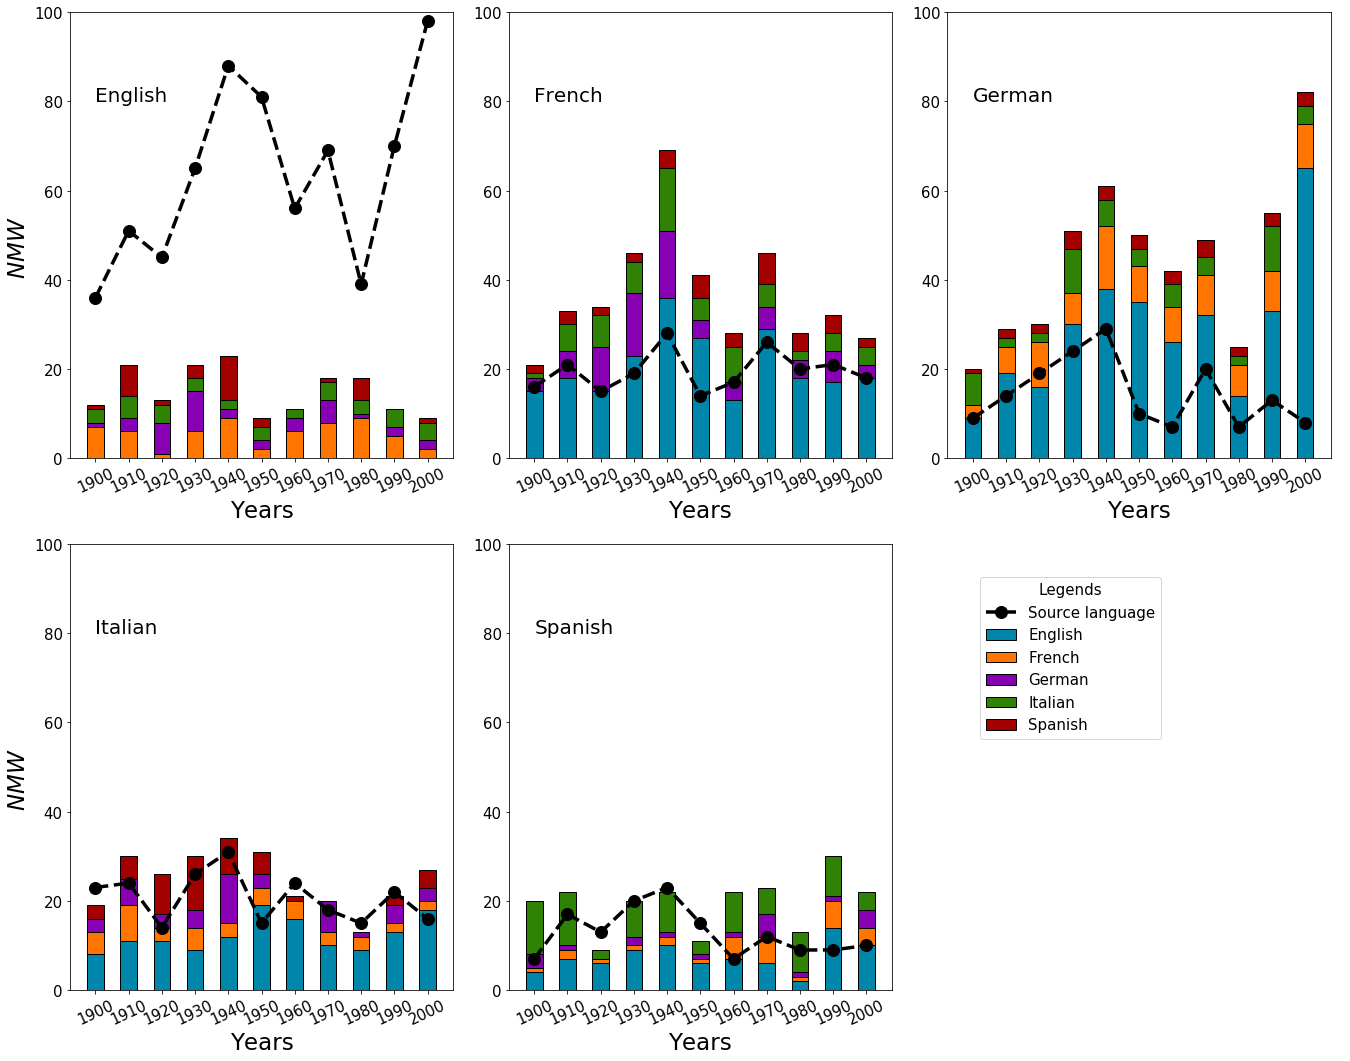
\includegraphics[scale=.35]{NW_A_ejes.png}
\caption{{\bf New migrant words, per language and per decade.} 
$NMW$ are consider for each language. Each panel contains one language. 
The dotted line displays the number of $NMW_{out}$ that originate in the 
corresponding language, and the bars the $NMW_{in}$ coming to that language, 
separated by the origin of the different $NMW$. }
% 
\label{fig.NMW_A}
\end{adjustwidth}
\end{figure} % }}}
	
Analyzing the lists  of 
% After counting, we analyzed each of the 
migrant words, we realized that
these can be grouped into semantic fields. According to~\cite{semantic_oxford},
a semantic field is a set of words that are related based on their meaning.
% then we can group the new migrant words by their meaning.
Table~\ref{tab.new_words} shows the words grouped by semantic fields, as well as
the pairs of source language and receiving language involved. We note that the
year of appearance (or in the years around) of the migrant words, a historical
or cultural event occurred that is related to the semantic field. For example,
between the 1930s and 1940s, words historically related to the Second World War
migrated between all languages; while since the 1990s, migrant words refer
to the fields of technology and globalization.  

\begin{table}[htb] % {{{
\centering
\resizebox{\textwidth}{!}{
\begin{tabular}{@{}cV{4.5}cV{4.5}cV{4.5}c@{}}
\textbf{Semantic Field} & \textbf{New migrant words}
      & \textbf{Source language} & \textbf{Receiving language (decade)} \\
\hlineB{4.5}
\multirow{2}{*}{World War I} 
   & \begin{tabular}[c]{@{}c@{}} \\ allemagne,  austro,\\  russie, versailles.\end{tabular} 
   & FR    & \begin{tabular}[c]{@{}c@{}}\\IT (1910, 1920), GE (1920).\end{tabular} \\
 & kaiser, reich. & GE   & FR (1910). \\
\hlineB{4.5}
	\multirow{5}{*}{World War II}                                                                    & \begin{tabular}[c]{@{}c@{}}catastrophe, churchill,\\ nazis, stalin, territories.\end{tabular}                                                           & EN                       & \begin{tabular}[c]{@{}c@{}}FR (1940), \\ IT (1940).\end{tabular}                                                     \\
	& \begin{tabular}[c]{@{}c@{}}berchtold, bestimmungen,\\  hitler, kaiser, lenin, \\ minister, regierung.\end{tabular}                                      & GE                       & \begin{tabular}[c]{@{}c@{}}EN (1930), FR (1940),\\ IT (1930, 1940),\\ SP (1930).\end{tabular}                        \\
	& \begin{tabular}[c]{@{}c@{}}duce, mussolini, \\ regime.\end{tabular}                                                                             & IT                       & \begin{tabular}[c]{@{}c@{}}EN (1930), FR (1930),\\ GE (1930, 1940),\\ SP (1930).\end{tabular}                        \\
	
	\hlineB{4.5}
	Aftermath of WWII                                                                                & onu, urss, vietnam                                                                                                                                      & FR                       & SP (1960, 1990).                                                                                                     \\
	\hlineB{4.5}
	\multirow{2}{*}{\begin{tabular}[c]{@{}c@{}}Historic figures\\ in arts, science\\ and philosophy \end{tabular}} & poincare.                                                                                                                                               & FR                       & IT (1920).                                                                                                           \\
	& \begin{tabular}[c]{@{}c@{}}bach, beethoven, engels, \\ freud, hegel, heidegger, \\ marx, mozart, nietzsche.\end{tabular}                                & GE                       & \begin{tabular}[c]{@{}c@{}}EN (1930), FR (1900-1980),\\ IT (1900, 1940, 1970),\\ SP (1930, 1970, 1980).\end{tabular} \\
	\hlineB{4.5}
	\multirow{2}{*}{\begin{tabular}[c]{@{}c@{}}Ideologies and \\ political terms\end{tabular}}       & \begin{tabular}[c]{@{}c@{}}burgueoise, diplomatie, \\ empire, politique.\end{tabular}                                                                   & FR                       & GE (1910-1930).                                                                                                      \\
	& \begin{tabular}[c]{@{}c@{}}capitalista, comunista, fascismo, \\ marxismo, socialista, terrorismo.\end{tabular}                                          & IT                       & SP (1910, 1930, 1960, 1980).                                                                                         \\
	
	
	\hlineB{4.5}
	Economy                                                                                          & \begin{tabular}[c]{@{}c@{}}depression, dollar, economic, \\ economy, financial, investment, \\ market, marketing, value.\end{tabular}                   & \multirow{4}{*}{EN}      & \begin{tabular}[c]{@{}c@{}}FR (1950), \\ GE (1930, 1990, 2000),\\ SP (1980-2000).\end{tabular}                       \\
	
	Technology                                                                                       & \begin{tabular}[c]{@{}c@{}}digital, internet, mail, \\ online, software.\end{tabular}                                                                   &                          & \begin{tabular}[c]{@{}c@{}}FR (1990), GE (1990),\\ IT (1990, 2000), \\ SP (1990, 2000).\end{tabular}                 \\
	Globalization                                                                                    & \begin{tabular}[c]{@{}c@{}}business, customer, management, \\ market, marketing, standars.\end{tabular}                                                 &                          & \begin{tabular}[c]{@{}c@{}}FR (2000), GE (1990, 2000),\\ IT (2000),  SP ( 2000).\end{tabular}                        \\
	\begin{tabular}[c]{@{}c@{}}Presidents of the\\ United States of\\p America\end{tabular}           & \begin{tabular}[c]{@{}c@{}}roosevelt, truman, kennedy,\\ johnson, nixon, reagan,\\ bush, clinton.\end{tabular}                                          &                          & \begin{tabular}[c]{@{}c@{}}FR (1960, 1970), GE (1930,1940),\\ IT (1940),  SP (1940-1990).\end{tabular}               \\
	\hlineB{4.5}
	Medicine                                                                                         & \begin{tabular}[c]{@{}c@{}}anemia, anestesia, colesterina,\\ endovenosa, gastrica, lepra\\ metabolismo, sintomatologia, virus,\\ vitamina.\end{tabular} & \multirow{2}{*}{SP}      & \begin{tabular}[c]{@{}c@{}}EN (1940), GE (1990,1940),\\ IT (1920, 1930),\end{tabular}                                \\
	\begin{tabular}[c]{@{}c@{}}Latinoamerican countries \\ and cities\end{tabular}                   & 
	\begin{tabular}[c]{@{}c@{}}argentina, aires, buenos,\\ chile, panama.\end{tabular}                                                                      &                          & \begin{tabular}[c]{@{}c@{}}EN (1910, 1940), FR (1910), \\ IT(1900).\end{tabular}                                    
\end{tabular}%
}
\caption{\textbf{New migrant words.} 
Examples of new migrant words for all pairs of languages, grouped together by semantic field.
A notorious influence of historic events on word migration is observed. 
We use the following abbreviations: EN for English, FR for French, GE for German, IT for
Italian and SP for Spanish. 
}
\label{tab.new_words}
\end{table} % }}}

These kind of groupings allow us to say in which areas the languages are most
influential and the reason for the migration of words. The English language has
migrated words to others because of technological development and
globalization in the last thirty years. French, Italian and German
were influential after the war events of the 20th century, in addition to the academic
influence of Germany seen through surnames of historic figures. Finally, Spanish was influential after economic crises in Latin American
countries~\cite{crisis_chile}. The fact that locations from one country become frequent words in another language suggests that some people speaking the latter are interested in the former. Similarly, influence can be seen e.g. as USA presidents become commonly used words (in the top 5000) in other languages. This suggests that migrant words could be used as a proxy measure of cultural influence (see next Section).

Another interesting feature that we observed is that migrant words also fulfill Zipf's law~\cite{Zipf}. In Fig~\ref{fig.ZL_receiving} we present all language pairs, grouped by receiving language and we observe (within fluctuations), an asymptotic power-law decay with an exponent close to one. 

\nrnote{The very last sentence of New Words reads “…within statistical
	fluctuations, an asymptotic power law decay with an exponent close to
	one.” What is meant by statistical fluctuations? That infers that
	there was a statistical model with a measure of variance. Was there a
	statistical model fit with these curves to evaluate the fit of a
	power-law decay}
	
\jmnote{Para la ley de zipf de las parejas de idiomas, se hizo un ajuste por el meotodo de minimos cuadrados para encontrar la ecuacion que ajuste los datos. La funcion que mejor ajusta es de la forma $f(k) = \alpha k^{\beta} $  donde los parametros $\alpha$ y $\beta$ se presentan en la tabla~\ref{tab.Ajustes Zipf}, donde ademas se calculo el ceoficiente de determinacion $R^{2}$ para medir la fiabilidad del ajuste. La formula para determinar R2 \[
	R^2 = 1 - \frac{\sum_{i=1}^{n} (y_i - \hat{y}_i)^2}{\sum_{i=1}^{n} (y_i - \bar{y})^2}
	\], donde $y_{i}$ es el valor real i-esimo de los datos, $\bar{y}$ el promedio de todos los datos, $\hat{y}_i$ el valor predicho i-esimo del ajuste }


\begin{table}
	\centering
	\begin{tabular}{ccccc}
		\toprule
		\thead{Idioma A} & \thead{Idioma B} & \thead{$\alpha$} & \thead{$\beta$} & \thead{ $R^{2}$ } \\
		\midrule
		FR & EN & 1.366 & -0.506 & 0.905 \\
		GE & EN & 0.984 & -1.149 & 0.994 \\
		IT & EN & 1.168 & -0.631 & 0.946 \\
		SP & EN & 1.201 & -0.580 & 0.946 \\
		Todos & EN & 1.180 & -0.716 & 0.000 \\
		EN & FR & 1.156 & -0.541 & 0.955 \\
		GE & FR & 1.033 & -0.802 & 0.985 \\
		IT & FR & 0.976 & -0.894 & 0.992 \\
		SP & FR & 1.261 & -0.646 & 0.910 \\
		Todos & FR & 1.106 & -0.721 & 0.000 \\
		EN & GE & 0.868 & -0.797 & 0.948 \\
		FR & GE & 1.345 & -0.496 & 0.878 \\
		IT & GE & 0.909 & -0.956 & 0.944 \\
		SP & GE & 1.140 & -0.630 & 0.936 \\
		Todos & GE & 1.066 & -0.720 & 0.000 \\
		EN & IT & 1.241 & -0.489 & 0.941 \\
		FR & IT & 1.260 & -0.613 & 0.905 \\
		GE & IT & 0.994 & -1.907 & 0.993 \\
		SP & IT & 1.068 & -0.740 & 0.985 \\
		Todos & IT & 1.141 & -0.937 & 0.000 \\
		EN & SP & 1.062 & -0.501 & 0.947 \\
		FR & SP & 1.002 & -1.141 & 0.988 \\
		GE & SP & 0.875 & -0.505 & 0.877 \\
		IT & SP & 1.276 & -0.596 & 0.947 \\
		Todos & SP & 1.054 & -0.686 & 0.000 \\
		\bottomrule
	\end{tabular}
	\caption{Tabla de ajustes Zipf}
	\label{tab.Ajustes Zipf}
\end{table}

%Another interesting feature that we observed is that migrant words also fulfill Zipf's law~\cite{Zipf}. In Fig~\ref{fig.ZL_receiving} we present all language pairs, grouped by receiving language and we observe, within statistical fluctuations, an asymptotic power-law decay with an exponent close to one.


%\cgnote{Se usa la frecuencia total de cada palabra migrante? para todos los años o para alguno en particular? Hay que explicar aqu\'i tambi\'en c\'omo se calcul\'o esa figura.}
% To answer how stable the sets are if we altering them, we first verify that in
% each year the accumulated migrant words between two languages, obey Zipf's law
% $f~1/k$ if they are order ascending by their rank Fig~\ref{fig.ZL_receiving};


\begin{figure}[!h]
	\begin{adjustwidth}{-2cm}{1cm}
		\centering
		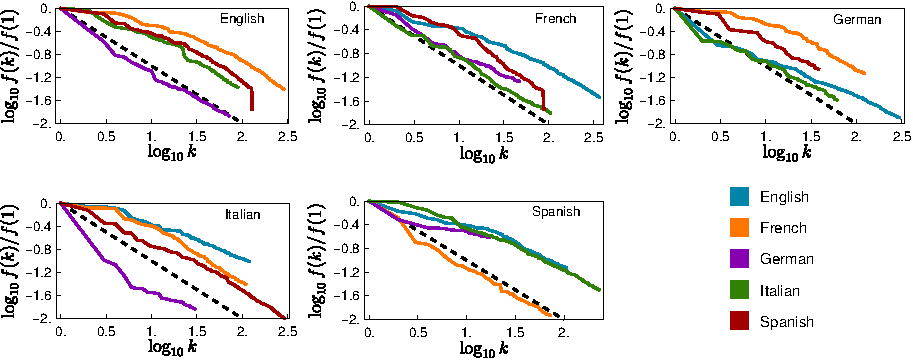
\includegraphics{images/zipfFinal.pdf}
% 		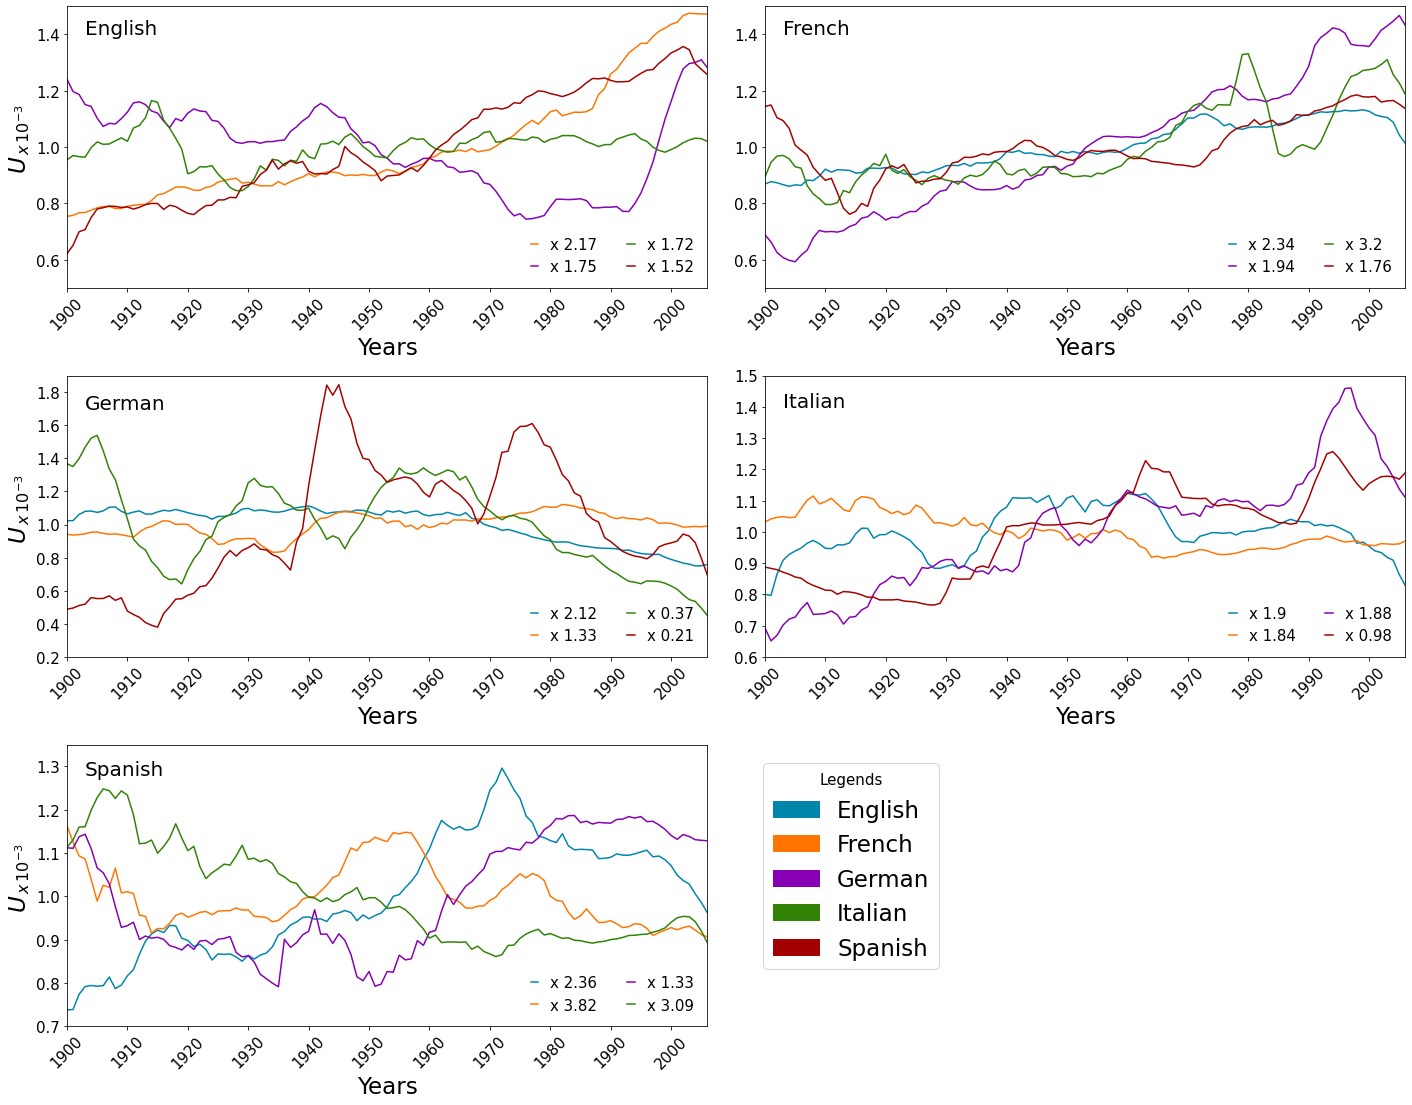
\includegraphics[scale=0.38]{USO_A.png}
		\caption{{\bf Zipf's law of the accumulated migrant words,
grouped by receiving language.} We display a frequency-rank 
plot for all language pairs, for the migrant words during the year 2000.
Indeed, after a transient, Zipf's law is observed (a dashed line with slope $-1$ is
provided for comparison). }
		\label{fig.ZL_receiving}
	\end{adjustwidth}
\end{figure}

% }}}
\section*{Accumulated words} % {{{
% Intro y definicion {{{

The previous results show that words travel from one language to another in
groups belonging to a common semantic field. Nevertheless, we still cannot
associate them with a number that quantifies how much influence has one
language on another.

To obtain such a number, we will focus on migrant words in the years after the
first year they migrated, observing how their frequency varies over time. For
example, a migrant word will begin to be influential if its frequency increases
over time. Since we are dealing with groups of words, we define as accumulated
migrant words, those words with source language $A$ that already appeared in a
receiving language $B$, and for a given year they do so again.


Consider the words that up to a given year $t$ have migrated from language $A$ to $B$. Each of these
words will have a ranking $f(j)$ where $j$ is the ranking of the word, within the aforementioned
list of words. 
% 
We now
add the frequencies of the accumulated
migrant words of $A$ to $B$ at a year $t$ and normalize the this quantity by
dividing it by the frequency of the first five thousand words that make up the list:
\begin{equation}
\label{ec.fuso}
\underset{ \text{\tiny A} \to  \text{\tiny B} }{U}(t) = \frac{\sum_{j}
f(j)}{\sum_{k=1}^{5000} f(k)}.
\end{equation}
We define this new value as the \textit{use} of $A$ in $B$, and interpret is value
as a measure of influence. It will then be said that the influence of $A$ has increased on
$B$, if in an interval of time $\Delta t$ the use of $A$ on $B$, $\underset{ \text{\tiny A} \to  \text{\tiny B} }{U}$, increases.

We obtained the accumulated migrant words for all possible combinations of
source and receiving languages from 1740 to 2009.  Afterwards, we calculated
the use, \eref{ec.fuso},  for each pair of languages between 1900 and 2009, so
as to have a time period (1740-1899) to build a large enough dataset to have
meaningful migrant words. The results are presented in \fref{fig.UT_art}, 
grouped by source language. 


% 
% Then in each combination we applied
% the equation~\ref{ec.fuso} to realize the use in the years between 1900 and
% 2009. 
% In addition, to name some combination of source
% and receiving languages, two abbreviations will be used, the first being the
% source language of the accumulated migrant words, and the second the receiving
% language of them, for example EN-GE, means the migrant words from English that
% are present in the German.


% To simplify the notation in the plots we establish a set of abbreviations to
% distinguish the languages: EN for English, FR for French, GE for German, IT for
% the Italian and SP for Spanish. In addition, to name some combination of source
% and receiving languages, two abbreviations will be used, the first being the
% source language of the accumulated migrant words, and the second the receiving
% language of them, for example EN-GE, means the migrant words from English that
% are present in the German.

% We obtained with the previous method, the accumulated migrant words among all
% the possible combinations from a source language to a receiving language, in
% the 269 years (1740-2009) of the dataset. Then in each combination we applied
% the equation~\ref{ec.fuso} to realize the use in the years between 1900 and
% 2009. To simplify the reading we establish s set of abbreviations to
% distinguish the languages, EN for English, FR for French, GE for German, IT for
% the Italian and SP for Spanish. In addition, to name some combination of source
% and receiving languages, two abbreviations will be used, the first being the
% source language of the accumulated migrant words, and the second the receiving
% language of them, for example EN-GE, means the migrant words from English that
% are present in the German.

% The migrant accumulated words between pairs of language were ordered by the
% year in which they appeared and in descending order in their frequency.
% Therefore the first place in the ranking is occupied by the most frequent word
% in that year, the second for the second most frequent, and so on.

% Fig~\ref{fig.UT_art} shows the use of a source language, in all receiving
% languages, as the use in each case may have a different scale, the data were
% normalized by dividing them by their average value, this with the intention of
% observing in which time interval the use was more affected (increase or
% decrease more than in the others), since this will indicate that accumulated
% words were more or less influential. 


\begin{figure}[!h]
	\begin{adjustwidth}{-2cm}{1cm}
		\centering
		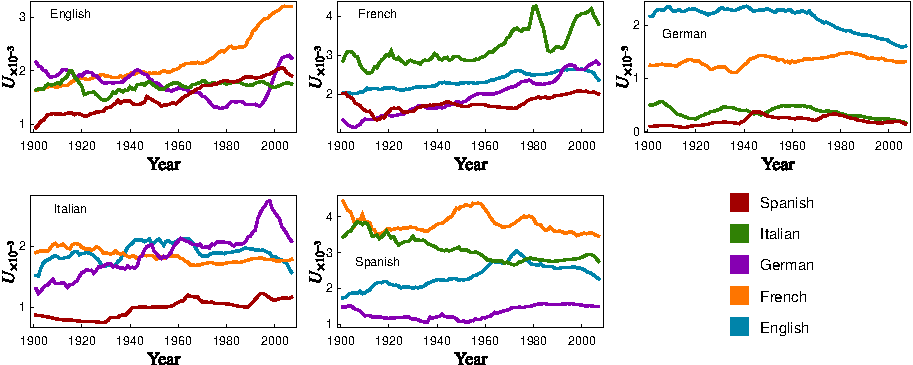
\includegraphics{images/usoFinal.pdf}
% 		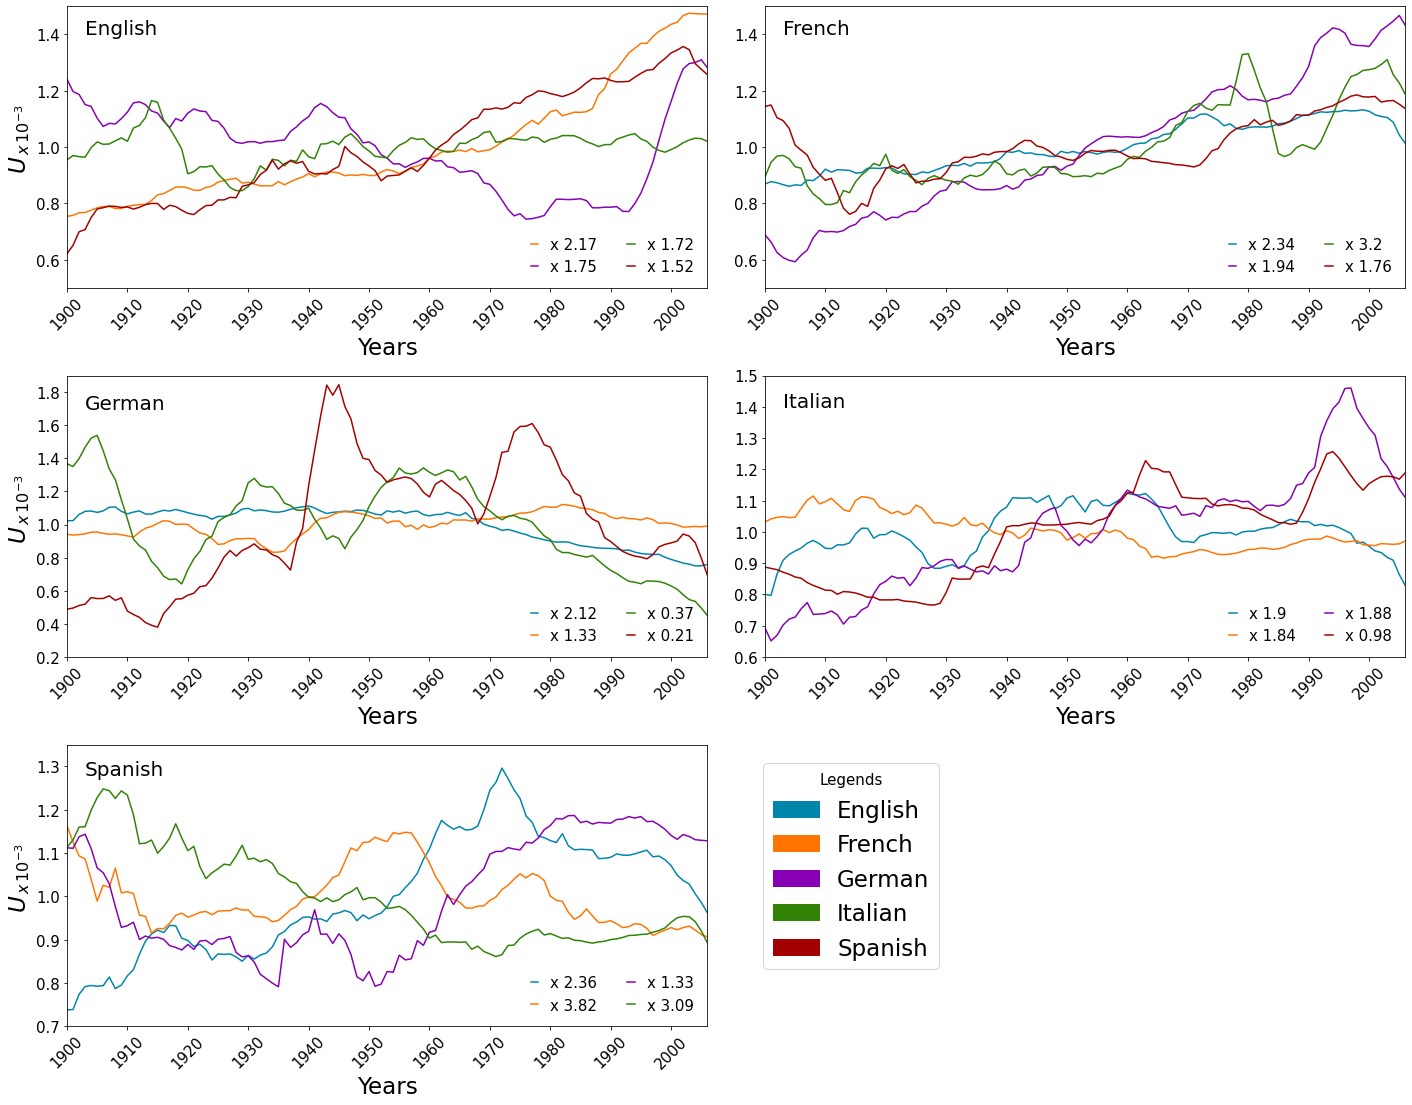
\includegraphics[scale=0.38]{USO_A.png}
		\caption{{\bf The use $U$ among languages.} 
We plot the use, as defined in \eref{ec.fuso} for all language pairs. 
Results are discussed in the
main text. }
		\label{fig.UT_art}
	\end{adjustwidth}
\end{figure}
% }}}
\subsubsection*{English} % {{{

The use of English in French and Spanish has increased steadily in the last century
whereas in Italian, it has maintained a constant level. 
\nrnote{In the English section under Accumulated Words it states that “the
	use of English in French and Spanish has increased steadily in the
	last century whereas in Italian, it has maintained a constant level.”
	This is an observational description of trends seen in the data and
	there is not a statistical model and analysis to evaluate if trends
	are constant or increasing at some rate. It would be nice to include
	those trend rates. The same is true for the French, German, Italian,
	and Spanish sections. }
\jmnote{Ver histogramas}
An increase of its use in German occurred after 1990, just after the fall of the Berlin Wall. We associate the cause of these increases
with the emergence of the United States as a world power, after the end of the
World War II, the propagation of its economic model, as well as the development
of science and technology. The accumulated migrant words that are present in all receiving
languages are \textit{capital}, \textit{dollar}, \textit{invesment},
\textit{relations}, \textit{market}, \textit{company}, \textit{development},
\textit{financial},  \textit{institutions}, \textit{internet}, \textit{windows}
and \textit{software}. Those can again be associated with semantic fields, such
as economics, technology, and globalization.

% }}}
\subsubsection*{French} % {{{

The increase of French influence in the other languages occurred in
English between 1920 and 1970, in German between 1900 and 2009, and in Spanish
between 1970 and 1995. In these years, words that increased their frequency
are from the semantic fields of religion such as \textit{dieu} ,
\textit{évêque}, \textit{dime}, \textit{religion}, \textit{saint} and
\textit{église} ; while \textit{reine}, \textit{forteresse},
\textit{napoleon}, \textit{guerre}, \textit{imperiale}, \textit{bastille},
\textit{royal} and \textit{bourgeois} have their roots in French history.

In Italian, between 1950 and 1970, in addition to the above
words, \textit{raisins}, \textit{vin}, \textit{vignoble} and \textit{recolte} were
found, the common meaning of which is the wine industry, a common industry in
France and Italy.

% }}}
\subsubsection*{German} % {{{

Spanish and French,  between 1930 and 1945, were the languages where German had the greatest
increase among all receiving languages. 
In both, the words that are present are the surnames of German-speaking
influential figures, such as \textit{Marx},
\textit{Freud}, \textit{Heidegger}, \textit{Nietzsche}, \textit{Hegel},
\textit{Engels} and \textit{Mozart}.

In English and Italian, the biggest change was between 1960 and 2009, where the
use of German decreased. In this period, some words that lost influence, in the
sense that their frequency decreased. 
Among these words are 
\textit{Berlin}, \textit{Marx},
\textit{Hitler}, \textit{Lenin}, \textit{testen}  and \textit{reich}.
% These words refer to the World War II, among them \textit{Berlin}, \textit{Marx},
% \textit{Hitler}, \textit{Lenin}, \textit{testen}  and \textit{reich}.
% }}}
\subsubsection*{Italian} % {{{


The influence of Italian came mainly from two semantic fields,  WWII with
\textit{Mussolini}, \textit{fascismo}, \textit{battaglia}, \textit{regime},
\textit{sociale}, and \textit{liberale}; and religion with \textit{santo},
\textit{suora} and \textit{cattedrale}. These semantic fields are
responsible for the increase in English between 1930 and 1940, in German
between 1950 and 1995, and in Spanish between 1930 and 1960.
A significant maximum of the influence of Italian in German is observed close to 1990. 
The words that produce such peak include 
\textit{usa},  \textit{tv}, and \textit{Rome}, which expose the limitation of our method. 
We think that the fact that 1990 FIFA World Cup final was played in Rome, where Germany won, might explain such behavior in the usage. 
% \textit{} 
% An inspection of the detected words 
% 

In French, Italian has the lowest influence, where the aforementioned words
began to be less frequent between 1940 and 1960.
% }}}
\subsubsection*{Spanish} % {{{

The influence of Spanish in English between 1920 and 1970, was due to
historical and cultural facts. Names of Latin American  countries such as
\textit{Mexico}, \textit{Panama}, \textit{Chile}, \textit{Cuba}, \textit{Peru},
\textit{Colombia}, \textit{Argentina} and its capital \textit{Buenos}
\textit{Aires};  and states that were previously Spanish colonies, and maintain Spanish names, such as \textit{California} and
\textit{Florida}, are an important part of words that appeared in 
other languages. 

In German after WWII, and in French between 1930 and 1955, the main words
involved in that increase are, \textit{terapia}, \textit{anemia},
\textit{lepra}, \textit{tumor}, \textit{syphilis}, \textit{virus}, and
\textit{renal}, related to the medical semantic field. 



% }}}
% }}}
\section*{Rank diversity} % {{{

In the previous sections, we quantified the influence of a language on another. However, 
one can wonder about how the migrant words change in time. Are the most important words
the same, or do they change? In fact, 
since the accumulated migrant words are organized by year, and at the same time
in each year the words are ordered in ascending order in rank, then over time,
the same rank can be occupied by different words. One way to quantify
this change is through rank diversity $d(k)$~\cite{iplosone}. This quantity is
defined as the number 
of different elements that occupied rank  $k$ within the same dataset, divided
by the number of time slots considered.
%  how many
% different elements can occupy the same rank within the same corpus is through
% rank diversity $d(k)$ 
% Since the accumulated migrant words are organized by year, and at the same time
% in each year the words are ordered in ascending order in rank, then over time,
% the same rank can be occupied by different words. One way to quantify how many
% different elements can occupy the same rank within the same corpus is through
Rank diversity has been used in datasets of the most used words in six
Indo-European languages~\cite{iplosone,10.3389/fphy.2018.00045,Cocho2019}, in sports and game classifications \cite{Morales_epj}, 
and in many other datasets~\cite{Iniguez2022}. 
Although in previous studies of rank diversity of languages and the current one the criteria for establishing rankings are different, in both there
is a common result: the lowest ranks are always occupied by fewer
elements, thereby as the rank increases, the number of different elements that occupied it
also does.

\begin{figure} % {{{
% \begin{adjustwidth}{-2.5cm}{1cm}
\centering
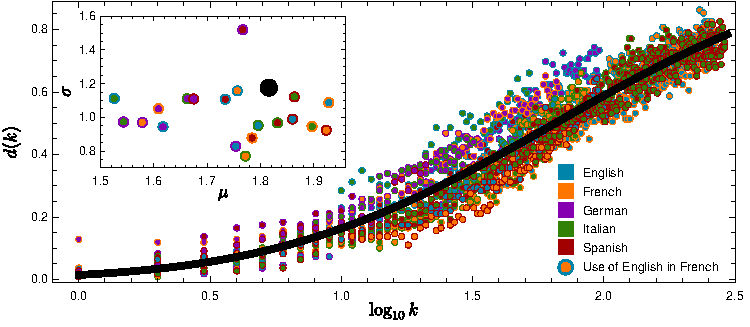
\includegraphics[scale=1]{images/Diversity.pdf}
% 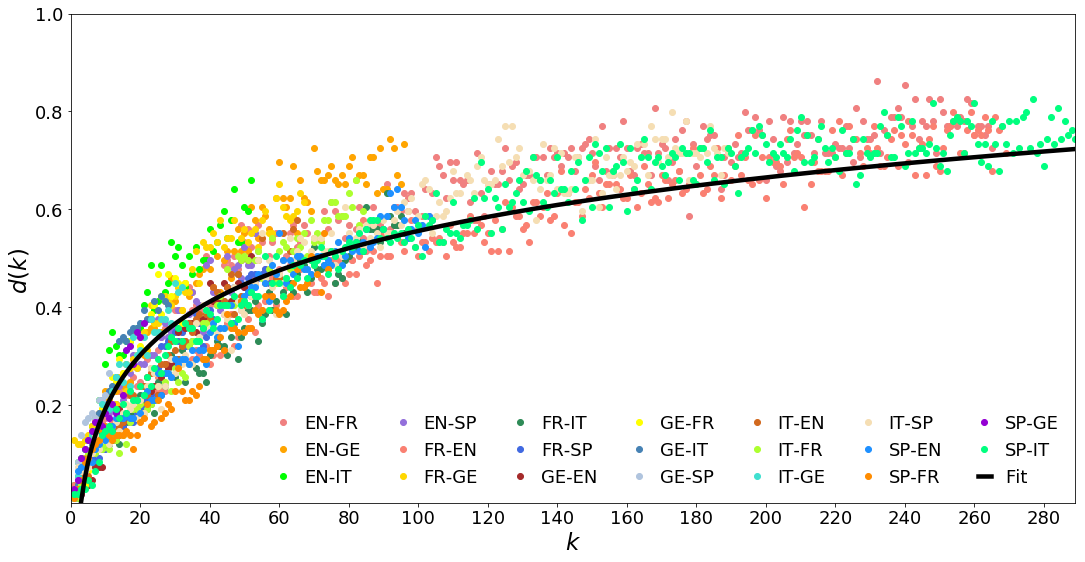
\includegraphics[scale=.38]{DR_art.png}
\caption{{\bf Rank diversity of accumulated migrant words among languages.} 
Diversity for all pairs of languages. Each pair is well fitted by the 
sigmoid proposed in \eref{eq:sigmoid}, with fitting parameters $\mu$ and $\sigma$
reported in the inset. As a reference, we show a global sigmoid (in black)
obtained by fitting all data points. Its fitting parameters are also shown in the
inset as a black dot. 
% 
% All
% language pairs conform the sigmoid curve proposed in 
% 
% 
%  show a logarithmic behavior regardless of the number of ranks
% where the rank diversity was applied. The reliability of the fit to a
% logarithmic curve of the 20 combinations is on average $R^{2}= 0.88 \pm 0.04$.
}
\label{fig.DR_art}
% \end{adjustwidth}
\end{figure} % }}}
After calculating the rank diversity (considering all years) for each source and receiving
language pair, the diversity values resemble a sigmoid curve, as can be
seen in Fig~\ref{fig.DR_art}. This can be fitted with a curve that is
cumulative of a Gaussian centered at $\mu$ and with 
deviation $\sigma$, i.e.  
\begin{equation}
\Phi_{\mu,\sigma}(\log_{10} k)=\frac{1}{\sigma\sqrt{2\pi}}
   \int_{-\infty}^{\log_{10}k}\exp\left(-\frac{(y-\mu)^2}{2\sigma^2}\right) {\rm d} y,
   \label{eq:sigmoid}
\end{equation}
The parameters $\mu$ and $\sigma$
are obtained with a linear regression. 
% If $ a_{k} $ represents the
% value of the adjustment equation when evaluating it in the range $ k $, $ d_
% {k} $ is the diversity obtained for the same range and $\bar{d} $ is the
% average of all values of the diversity, then
% $R^{2}=1-\sum_{k=1}(d_k-a_k)^{2}/(d_k-\bar{d})^2$.	
% Fig~\ref{fig.DR_art} also shows the plot of $d(k) = 0.16\ln(k) -
% 0.17$, obtained after averaging the coefficients $\alpha$ and $\beta$
% corresponding to each language pair. 
It is observed that the behavior of
diversity increases as the rank also increases, regardless of whether the
corpus has few or many ranks ($14$ in German-Spanish, $290$ in Spanish-Italian,
etc). With this, it can be concluded that, the migrant accumulated words in the
middle and high ranks are the ones that tend to change their position the most
within a ranking over time.

These observations suggest that only (relatively) few migrant words are used frequently, during long periods of time, while most migrant words are used not so (relatively) frequently, and their usage varies (relatively) more with time. 

% An final observation is that 
% The method of the use of one language in another, showed that
% the words of certain semantic fields decrease their rank if the use tends to
% increase.
% Nevertheless, the inverse case cannot be concluded, that is, we do not know if
% the use of a language increases as a consequence of a group of words decreasing
% its rank, nor do we know how stable is the use among languages if certain words
% were not taken; since within the accumulated words of one language in another,
% only a few belong to a specific semantic field.


% }}}
\section*{Robustness} % {{{
The method we used to build the set of migrant words relied on words having {\it
exactly} the same spelling when going from one language to another. We know 
that that is not always the case. Some words change their spelling. For example
the word {\it parquear} in Spanish comes from to the verb {\it to park} in
English. 


To check the stability of the results presented and the importance of omitting
certain words, we proceeded as follows:  Take the original set (the one
used in the previous section) of the accumulated words of a pair of source
language and receiving language. From this set, eliminate a certain group
of words, in order to obtain a reduced set; in both,  equation~\ref{ec.fuso} is
used to obtain the modified use between the years 1900 and 2009.  The next
thing is to determine how similar the use of both sets are. We normalized the
values of both sets, after dividing them by the average value of each one; then
for each year $t$ we obtain the distance between each value of original use
$u_{t}$ and its corresponding value in reduced use $r_{t}$. The average of them
gets the \textit{average distance} $\left\langle D \right\rangle$, which will
be the one that quantifies the similarity of the results, indicating a greater
similarity if it is close to zero. This distance is defined as 
\begin{equation}
\left\langle D \right\rangle  = \frac{1}{N}\sum_{t=1}^{N} \left| u_{t} - \tilde u_{t} \right|  
\label{ec.Davg}
\end{equation}
where $u(t)$ is the original normalized usage and $\tilde u(t)$ is the reduced,
normalized usage.

% \subsection*{Elimination characteristics}



Recalling that migrant words have frequency inversely proportional to the rank,
it is clear that some words are more important than others (see
\fref{fig.ZL_receiving}).  Thus, care must be taken when one removes a fixed
proportion of words, or a fixed frequency, as it can cause a big difference. 
One way to explore such aspect is to remove words from higher ranks
or lower ranks. 
% In particular, we consider two sets, 
With these ideas, in each source language
and receiving language pair, we carry out two types of elimination, in the
first we begin to eliminate the words with the lowest ranks gradually 
increasing the proportion of words removed $R_{p}$ (from 1$\%$ to a
99$\%$); in the opposite way, for the second case,  we begin by
eliminating those words with highest ranks. In both cases,
each time the eliminated portion was increased, the average difference was
calculated to observe the similarity.


\begin{figure}[!h]
	\begin{adjustwidth}{-2.5cm}{1cm}
		\centering
		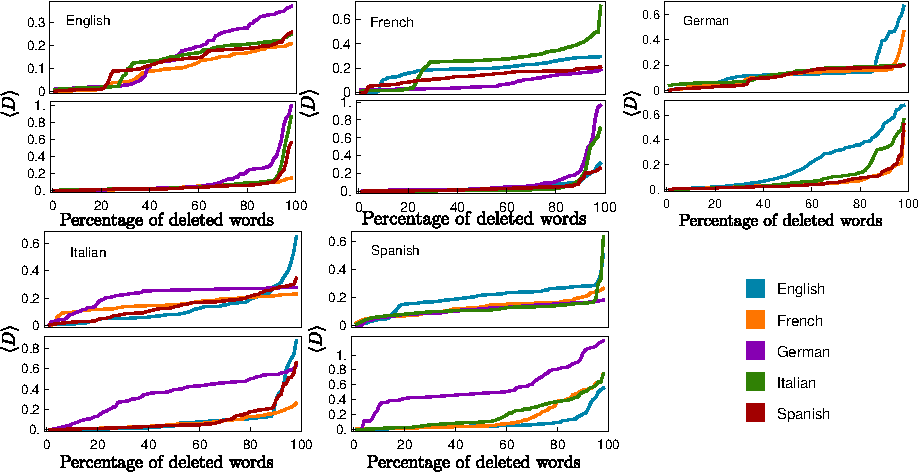
\includegraphics{images/dsFinal}
% 		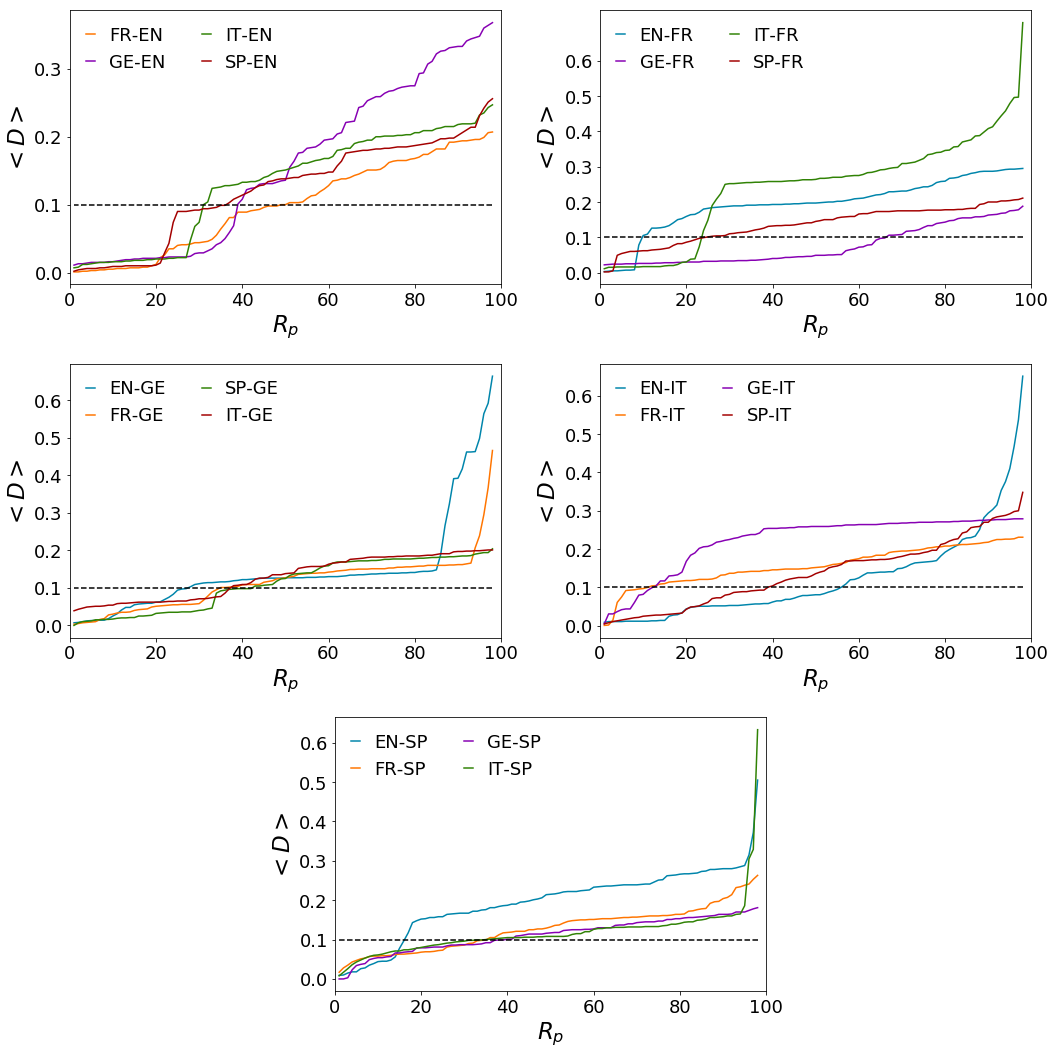
\includegraphics[scale=.38]{Rp_bajos.png}
		\caption{{Similarity of use when some words are eliminated.}
We study the similarity of the shape of usage \eref{ec.fuso}, as measured by
$\left\langle D \right\rangle $ (see \eref{ec.Davg}), when some words are eliminated.
The upper plots correspond to the case in which the lower ranked words (more frequent) are being
eliminated first, whereas in the lower plots we start eliminating the higher ranked
words (less frequent). 
% {\bf Portion of eliminated words with lows ranks.}{\bf Portion of eliminated
% words with high ranks.} 
}
		\label{fig.RP}
	\end{adjustwidth}
\end{figure}


% \begin{figure}[!h]
% 	\begin{adjustwidth}{-2.5cm}{1cm}
% 		\centering
% 		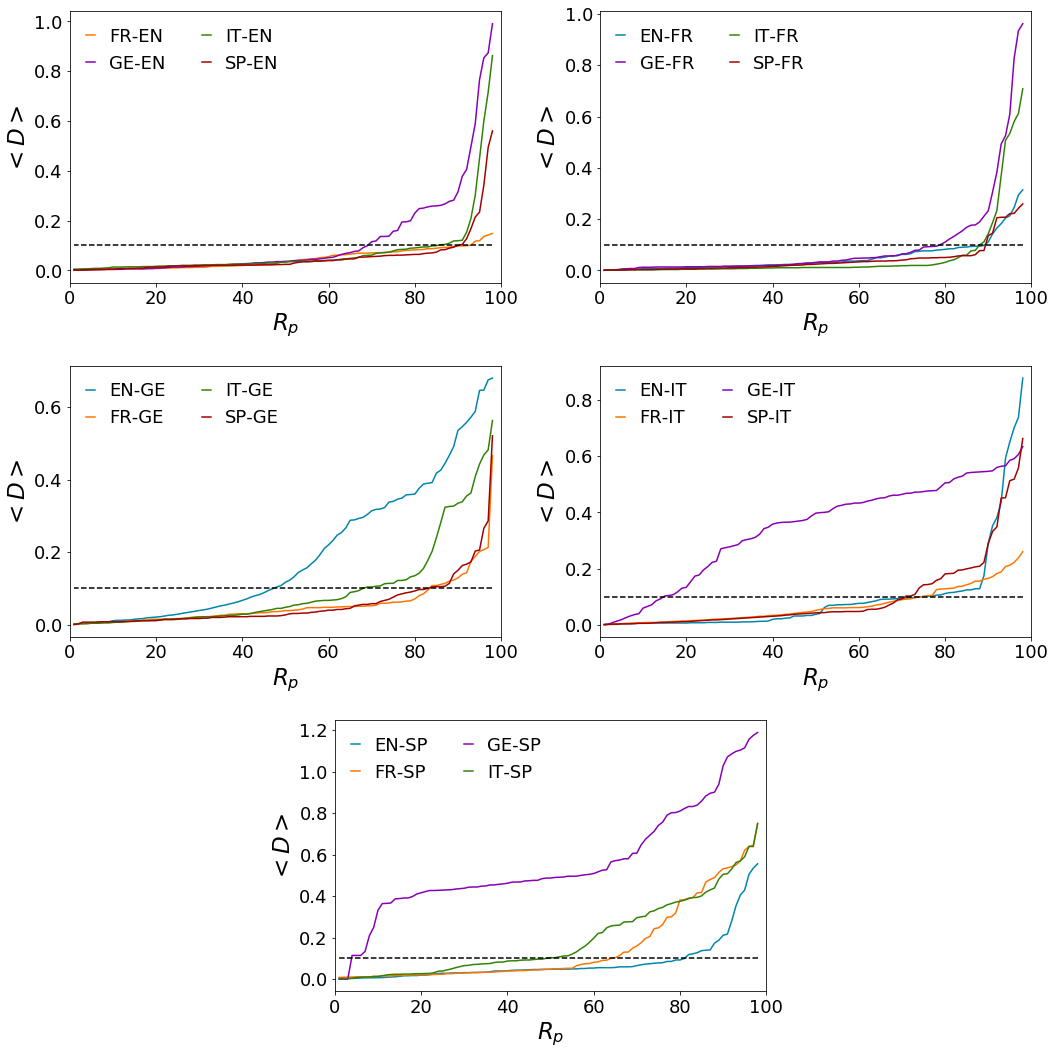
\includegraphics[scale=.38]{Rp_altos.png}
% 		\caption{{\bf Portion of eliminated words with high ranks.} }
% 		\label{fig.RP_high}
% 	\end{adjustwidth}
% \end{figure}
% 

In Fig.~\ref{fig.RP} we can observe how much the shape of the curves for usage changes, 
with an increasing proportion of words eliminated. Clearly, when removing the 
lower ranking words, the deformation is greater. However, we see that in 
most cases,  removing the 60\% of the higher ranked words produces
a deformation with $\langle D \rangle < 10\%$ (exceptions being 
German influencing English, Italian influencing German and
Spanish influencing German and Italian). 
% 
% 
% 
% After observing both figures, it is appropriate to say that for the similarity
% of the use between languages are altered, a greater number of words with high
% ranks are needed than words with low ranks, in terms of robustness, the sets
% are more stable if altering them are eliminated those words with the highest
% ranks, that is, those with the lowest frequencies.
% 
This result implies that care must be taken when doing this analysis with respect to 
words that have low ranks. Thus, using this automated approach
to yield quantitative statements should pay special attention to the most frequently used words. 

% \cgnote{Question: why the upper figures do not have a maximum at 100\% equal to the lower figures? shouldn't the distances be the same once you removed all migrant words? Also, it was not clear to me whether the distance was taken only between sets of migrant words, or all words (as you remove only migrant words)}
% 
% \jmnote{Para la robustes se eliminaron palabras migrantes de un idioma en otro,
% y a partir de la eliminacion se calculo el uso ec1. Con ello ya se tienen dos
% curvas una original (con las frecuencias de todas las palabras migrantes) y
% otra que es una fraccion o porcion de ella (algunas frecuencias de las palabras
% migrantes); para ver que tan similares son se normalizo cada una por su valor
% promedio y se calculo ec3. La razon de que las graficas no esten con la misma
% escala esque la normalizacion del promedio no ajusta los valores entre cero y
% uno, solo sabemos que entre mas pequeña sea la distancia la similitud es mejor.
% }
% , despite showing the stability of the sets when eliminating words
% from them, can be counterproductive with the results of the
% previous sections, since in those we try to find relationships based on the
% meaning of the words, and in case of an elimination such relationships would be
% lost if the words involved have high ranks.

%just multiply the original use by the conversion factor to obtain the reduced use. 

% }}}
\section*{Discussion} % {{{

We presented a method and analyzed how migrant words (loanwords with the same spelling) have spread across five Indoeuropean languages. This ``blind big data'' approach can offer some insights, so as to estimate influences in different temporal periods, and how historic events might have contributed to these fluxes. Nevertheless, our method has important caveats. As it is, it requires that languages use the same alphabet (although some automatic transliteration could be used to include more languages, such as Russian). However, languages also change the spelling of words as they migrate from one to the other. For example, in Spanish it is difficult to pronounce words beginning with `s' followed by a consonant, so an `e' is added (e.g., `especial', `espectacular', `estable'; although these come from Latin, not English). Indeed, some words might have their origins in a language not considered in a specific study, e.g. `sushi', although it might be useful to learn in which languages such words became popular first, even when it is uncertain whether the word migrated directly from the original to others, or via an intermediary (such as Nahuatl words that have spread globally through Spanish, e.g. `tomatl', `xocolatl'). Still, as more data becomes available, more languages could be included in statistical studies. Another limitation of our present work is that we focus on frequently used words, although the same methodology could be used for less frequent words as well. These caveats imply that we are not attempting to replace ``insightful small data'' studies, where experts focus on particular words and study how they are shared across languages. We believe that both types of studies are complementary and necessary.

Additionally from the linguistic aspects of these studies, they can be useful to study cultural influence as well. The fact that a name of a place or person from one place is used frequently in another implies relevance. Thus, migrant words can be used also as proxies of cultural influence.

More sophisticated statistical linguistic studies are becoming possible because of increasing data availability and computational processing power. Still, we must be aware of the limitations of these methods. They can offer useful insights, complementary to but not replacing other approaches in linguistics and culturomics~\cite{Michel14012011,doi:10.1073/pnas.2102061118}.

% }}}
\section*{Supporting information} % {{{
% }}}
\section*{Acknowledgments} % {{{

\nolinenumbers
We are grateful for stimulating conversations with Sergio Sanchez during the onset of this project.  Support by projects CONACyT 285754 and UNAM-PAPIIT (IG101421, IN107919, IV100120, IN105122) and from the PASPA program from UNAM-DGAPA is acknowledged. 
% }}}
\bibliography{referencias} 
\end{document}
